\newcommand{\svcourse}{CST Part IA: Software Engineering and Security}
\newcommand{\svnumber}{1}
\newcommand{\svvenue}{Microsoft Teams}
\newcommand{\svdate}{2022-05-11}
\newcommand{\svtime}{15:00}
\newcommand{\svuploadkey}{CBd13xmL7PC1zqhNIoLdTiYUBnxZhzRAtJxv/ytRdM1r7qIfwMsxeVwM/pPcIo8l}

\newcommand{\svrname}{Dr Sam Ainsworth}
\newcommand{\jkfside}{oneside}
\newcommand{\jkfhanded}{yes}

\newcommand{\studentname}{Harry Langford}
\newcommand{\studentemail}{hjel2@cam.ac.uk}


\documentclass[10pt,\jkfside,a4paper]{article}

% DO NOT add \usepackage commands here.  Place any custom commands
% into your SV work files.  Anything in the template directory is
% likely to be overwritten!

\usepackage{fancyhdr}

\usepackage{lastpage}       % ``n of m'' page numbering
\usepackage{lscape}         % Makes landscape easier

\usepackage{verbatim}       % Verbatim blocks
\usepackage{listings}       % Source code listings
\usepackage{graphicx}
\usepackage{float}
\usepackage{epsfig}         % Embed encapsulated postscript
\usepackage{array}          % Array environment
\usepackage{qrcode}         % QR codes
\usepackage{enumitem}       % Required by Tom Johnson's exam question header

\usepackage{hhline}         % Horizontal lines in tables
\usepackage{siunitx}        % Correct spacing of units
\usepackage{amsmath}        % American Mathematical Society
\usepackage{amssymb}        % Maths symbols
\usepackage{amsthm}         % Theorems

\usepackage{ifthen}         % Conditional processing in tex

\usepackage[top=3cm,
            bottom=3cm,
            inner=2cm,
            outer=5cm]{geometry}

% PDF metadata + URL formatting
\usepackage[
            pdfauthor={\studentname},
            pdftitle={\svcourse, SV \svnumber},
            pdfsubject={},
            pdfkeywords={9d2547b00aba40b58fa0378774f72ee6},
            pdfproducer={},
            pdfcreator={},
            hidelinks]{hyperref}

\renewcommand{\headrulewidth}{0.4pt}
\renewcommand{\footrulewidth}{0.4pt}
\fancyheadoffset[LO,LE,RO,RE]{0pt}
\fancyfootoffset[LO,LE,RO,RE]{0pt}
\pagestyle{fancy}
\fancyhead{}
\fancyhead[LO,RE]{{\bfseries \studentname}\\\studentemail}
\fancyhead[RO,LE]{{\bfseries \svcourse, SV~\svnumber}\\\svdate\ \svtime, \svvenue}
\fancyfoot{}
\fancyfoot[LO,RE]{For: \svrname}
\fancyfoot[RO,LE]{\today\hspace{1cm}\thepage\ / \pageref{LastPage}}
\fancyfoot[C]{\qrcode[height=0.8cm]{\svuploadkey}}
\setlength{\headheight}{22.55pt}


\ifthenelse{\equal{\jkfside}{oneside}}{

 \ifthenelse{\equal{\jkfhanded}{left}}{
  % 1. Left-handed marker, one-sided printing or e-marking, use oneside and...
  \evensidemargin=\oddsidemargin
  \oddsidemargin=73pt
  \setlength{\marginparwidth}{111pt}
  \setlength{\marginparsep}{-\marginparsep}
  \addtolength{\marginparsep}{-\textwidth}
  \addtolength{\marginparsep}{-\marginparwidth}
 }{
  % 2. Right-handed marker, one-sided printing or e-marking, use oneside.
  \setlength{\marginparwidth}{111pt}
 }

}{
 % 3. Alternating margins, two-sided printing, use twoside.
}


\setlength{\parindent}{0em}
\addtolength{\parskip}{1ex}

% Exam question headings, labels and sensible layout (courtesy of Tom Johnson)
\setlist{parsep=\parskip, listparindent=\parindent}
\newcommand{\examhead}[3]{\section{#1 Paper #2 Question #3}}
\newenvironment{examquestion}[3]{
\examhead{#1}{#2}{#3}\setlist[enumerate, 1]{label=(\alph*)}\setlist[enumerate, 2]{label=(\roman*)}
\marginpar{\href{https://www.cl.cam.ac.uk/teaching/exams/pastpapers/y#1p#2q#3.pdf}{\qrcode{https://www.cl.cam.ac.uk/teaching/exams/pastpapers/y#1p#2q#3.pdf}}}
\marginpar{\footnotesize \href{https://www.cl.cam.ac.uk/teaching/exams/pastpapers/y#1p#2q#3.pdf}{https://www.cl.cam.ac.uk/\\teaching/exams/pastpapers/\\y#1p#2q#3.pdf}}
}{}


\usepackage{mathtools}
\usepackage{tikz}
\usepackage{float}
\usepackage{graphicx}
\usepackage{wasysym}
\usepackage{ebproof}
\usepackage{rotating}

\begin{document}

\section{Notes Page 32}

\begin{enumerate}

\item Write a program to compute the factorial of the integer initially in
location $\ell_1$.

\[
\begin{split}
\langle&\ell_2 \coloneqq \ !\ell_1;\\
&\ell_{3} \coloneqq 1; \\
&\text{While}(!\ell_2 \geq 1) \\
&\text{do}( \\
&\ \ \ \ \ell_4 \coloneqq \ !\ell_2; \\
&\ \ \ \ \ell_5 \coloneqq 0; \\
&\ \ \ \ \text{While}(!\ell_4 \geq 1) \\
&\ \ \ \ \text{do}( \\
&\ \ \ \ \ \ \ \ \ell_5 \coloneqq \ !\ell_5 + \ !\ell_3; \\
&\ \ \ \ \ \ \ \ \ell_4 \coloneqq \ !\ell_4 + -1 \\
&\ \ \ \ ) \\
&\ \ \ \ \ell_3 \coloneqq \ !\ell_5; \\
&\ \ \ \ \ell_2 \coloneqq \ !\ell_2 + -1 \\
&), \\
&\{\\
&\ \ \ \ \ell_1 \mapsto n,\\
&\ \ \ \ \ell_2 \mapsto 0,\\
&\ \ \ \ \ell_3 \mapsto 0,\\
&\ \ \ \ \ell_4 \mapsto 0,\\
&\ \ \ \ \ell_5 \mapsto 0,\\
&\}\rangle
\end{split}
\]

\setcounter{enumi}{2}

\item Give full derivations of the first four reduction steps of the
$\langle e, s\rangle$ of the first L1 example on slide 22
\begin{gather*}
\frac{\overline{\langle\ell_0\coloneqq 7, \{\ell_0\mapsto 0,
\ell_1\mapsto0\}\rangle \to \langle\text{skip}, \{\ell_0\mapsto 7,
\ell_1\mapsto0\}\rangle}}{\langle(\ell_0 \coloneqq 7);(\ell_1 \coloneqq(!\ell_0 +2)),
\{\ell_0\mapsto 0, \ell_1\mapsto0\}\rangle\to\langle\text{skip};
(\ell_1 \coloneqq (!\ell_0 + 2)),\{\ell_0\mapsto 7, \ell_1\mapsto0\}\rangle}\\
\\
\frac{\overline{\langle \text{skip}; e, \emptyset
\rangle\to\langle e, \emptyset\rangle}}{\langle\text{skip};
(\ell_1 \coloneqq (!\ell_0 + 2)),\{\ell_0\mapsto 7, \ell_1\mapsto0\}\rangle\to
\langle\ell_1 \coloneqq (!\ell_0 + 2),\{\ell_0\mapsto 7, \ell_1\mapsto0\}\rangle}\\
\\
\frac{\overline{\langle!\ell_0,
\{\ell_0\mapsto7\}\rangle\to \langle7,
\{\ell_0\mapsto7\}\rangle}}{\langle(\ell_1 \coloneqq
(!\ell_0 + 2)),\{\ell_0\mapsto 7,
\ell_1\mapsto0\}\rangle\to\langle (\ell_1 \coloneqq (7 + 2)),
\{\ell_0\mapsto 7,
\ell_1\mapsto0\}\rangle}\\
\\
\frac{\overline{\langle7 + 2, \emptyset\rangle\to \langle 9,
\emptyset\rangle}}{\langle
(\ell_1 \coloneqq
(7 + 2)), \{\ell_0\mapsto 7,
\ell_1\mapsto0\}\rangle\to\langle (\ell_1 \coloneqq 9),
\{\ell_0\mapsto 7,
\ell_1\mapsto0\}\rangle}\\
\end{gather*}

\item Adapt the implementation code to correspond to the two rules (op1b)
and (op2b) on slide 44. Give some test cases that distinguish between the
original and the new semantics.

To change the implementation such that it corresponds to op1b and op2b, we
need to change only the match case for \texttt{Op} -- this involves changing
9 characters:

\begin{lstlisting}[language=Caml]
...
let rec reduce (e, s) =
  match e with
  ...
  | Op (e1,opr,e2) ->
      (match (e1,opr,e2) with
      ...
      | (e1,opr,e2) -> (
          if (is_value e2) then
            (match reduce (e1,s) with
            | Some (e1',s') -> Some (Op(e1',opr,e2),s')     (* (op2b) *)
            | None -> None )
          else
            (match reduce (e2,s) with
            | Some (e2',s') -> Some(Op(e1,opr,e2'),s')      (* (op1b) *)
            | None -> None ) ) )
...
\end{lstlisting}

The following code samples would differentiate between the cases:

\begin{gather*}
    \langle !\ell + (\ell \coloneqq 1; 1), \{\ell \mapsto 0\} \rangle\\
    \langle \text{while} \ (!x \geq (x \coloneqq !x - 1; 0)) \text{ do } (y \coloneqq !y + !x)
\rangle\\
\end{gather*}

\setcounter{enumi}{7}

\item Give a type derivation for $e$ on slide 32 with $\Gamma =
\ell_1:\text{intref}, \ell_2:\text{intref}, \ell_3:\text{intref}$.

Done on next page.

\begin{sidewaysfigure}
\begin{prooftree}
\hypo{\begin{matrix}\Gamma\vdash 0: \text{int}\\\Gamma(\ell_2)
=\text{intref}\end{matrix}}
\Infer1[(assign)]{\Gamma\vdash \ell_2 \coloneqq 0:\text{int}}

\hypo{\Gamma\vdash-1:\text{int}}
\hypo{\Gamma(\ell_1):\text{intref}}
\Infer1[(deref)]{\Gamma\vdash!\ell_1:\text{int}}
\Infer2[(op$\geq$)]{\Gamma\vdash!\ell_1\geq 1:\text{bool}}

\hypo{\Gamma(\ell_2):\text{intref}}
\Infer1[(deref)]{\Gamma\vdash !\ell_2:\text{int}}
\hypo{\Gamma(\ell_1):\text{intref}}
\Infer1[(deref)]{\Gamma\vdash !\ell_1:\text{int}}
\Infer2[(op+)]{\Gamma\vdash!\ell_1 + !\ell_2:\text{int}}
\Infer1[(assign)]{\Gamma\vdash\ell_2\coloneqq!\ell_1 + !\ell_2: \text{int}}

\hypo{\Gamma\vdash -1: \text{int}}
\hypo{\Gamma(\ell_1):\text{intref}}
\Infer1[(deref)]{\Gamma\vdash !\ell_1:\text{int}}
\Infer2[(op+)]{\Gamma\vdash !\ell_1 + -1: \text{int}}
\Infer1[(assign)]{\Gamma\vdash\ell_1\coloneqq !\ell_1 + -1: \text{unit}}
\Infer2[(seq)]{\Gamma\vdash\ell_2\coloneqq!\ell_2+\ell_1;
\ell_1\coloneqq!\ell_1+-1: \text{unit}}
\Infer2[(while)]{\Gamma \vdash \text{While}(!\ell_1 \geq 1)\text{ do }
(\ell_2 \coloneqq !\ell_2 + !\ell_1; \ell_1 \coloneqq !\ell_1 + -1)
:\text{unit}}
\Infer2[(seq)]{\Gamma \vdash \ell_2 \coloneqq 0; \text{While}(!\ell_1 \geq 1)
\text{ do }
(\ell_2 \coloneqq !\ell_2 + !\ell_1; \ell_1 \coloneqq !\ell_1 + -1)
:\text{unit}}
\end{prooftree}

\end{sidewaysfigure}

\newpage

\iffalse

\begin{tikzpicture}
\draw (-6, 0.4) -- (7.5, 0.4);
\draw (-2.5, 1.2) -- (7.5, 1.2);
\draw (-2.4, 2) -- (0.4, 2);
\draw (0.7, 2) -- (8.5, 2);
\draw (0.7, 2.8) -- (4.3, 2.8);
\draw (4.7, 2.8) -- (8.3, 2.8);
\draw (0.6, 3.6) -- (4.4, 3.6);
\draw (4.6, 3.6) -- (8.4, 3.6);
\node[anchor=center] at (-4.5, 0.8) {$\Gamma \vdash \ell_2 \coloneqq 0:
\text{unit}$};
\node[anchor=center] at (-1, 2.4) {$\Gamma \vdash !\ell_1: \text{int}$};
\node[anchor=center] at (-1, 1.6) {$\Gamma \vdash !\ell_1 \geq 1:
\text{bool}$};

\node[anchor=center] at (1.5, 4) {$\Gamma \vdash !\ell_2: \text{int}$};
\node[anchor=center] at (3.5, 4) {$\Gamma \vdash !\ell_1: \text{int}$};
\node[anchor=center] at (2.5, 3.2) {$\Gamma \vdash !\ell_2 + !\ell_1:
\text{int}$};
\node[anchor=center] at (2.5, 2.4) {$\Gamma \vdash \ell_2 \coloneqq !\ell_2 +
!\ell_1: \text{unit}$};

\node[anchor=center] at (7.5, 4) {$\Gamma \vdash !\ell_1: \text{int}$};
\node[anchor=center] at (5.5, 4) {$\Gamma \vdash -1: \text{int}$};
\node[anchor=center] at (6.5, 3.2) {$\Gamma \vdash !\ell_1 + -1: \text{int}$};
\node[anchor=center] at (6.5, 2.4) {$\Gamma \vdash \ell_1 \coloneqq !\ell_1 +
-1: \text{unit}$};

\node[anchor=center] at (4.5, 1.6) {$\Gamma \vdash \ell_2 \coloneqq !\ell_2 +
!\ell_1; \ell_1 \coloneqq !\ell_1 + -1: \text{unit}$};

\node[anchor=center] at (2.5, 0.8) {$\Gamma \vdash \text{While} (!\ell_1
\geq 1)
\text{ do }(\ell_2 \coloneqq !\ell_2 + !\ell_1; \ell_1 \coloneqq !\ell_1 +
-1): \text{unit}$};

\node[anchor=center] at (0, 0) {$\Gamma \vdash ; \ell_2 \coloneqq 0;
\text{While} (!\ell_1 \geq 1) \text{ do }(\ell_2 \coloneqq !\ell_2 + !\ell_1;
 \ell_1 \coloneqq !\ell_1 + -1): \text{unit}$};

\end{tikzpicture}
\fi

\item Does Type preservation hold for the variant language with rules
\texttt{assign1}\('\) and \texttt{seq1}\('\) on slide 45? If not, give an example and
show how type rules could be adjusted to make it true.

Type preservation does not hold for the variant language with rules
\texttt{assign1}$'$ and \texttt{seq1}$'$. This is because the type
returned from assignment is still \texttt{unit}.

In the modified language, programs such as $\langle \ell \coloneqq (\ell \coloneqq 0) + 1,
\{\ell\mapsto 0\}\rangle$ are valid. However, the typing rules would reject
this program! The type of $\ell \coloneqq 0$ would be \texttt{unit} -- we cannot
add a value of type unit and an integer so the program would be rejected
under the previous typing rules..

This can be resolved by changing the type derivation rule for
\texttt{assign1}$'$ to:

\[
\dfrac{\Gamma(\ell) = \text{intref} \ \ \ \Gamma \vdash e: \text{int}}{\Gamma
\vdash\ell \coloneqq e: \text{int}}
\]

\end{enumerate}

\section{Notes Page 49}

\begin{enumerate}

\setcounter{enumi}{11}

\item Without looking at the proof in the notes, do the cases of the proof
of Theorem 1 (Determinacy) for $e_1 \text{ op } e_2$ and
$\text{while } e_1 \text{ do } e_2$.

We can prove Determinacy using Structural induction.

Define $\Phi(e)$ as the expression $e$ is deterministic:
\[
\Phi(e) \triangleq \forall e, e', s, s', s'' (\langle e, s \rangle
\to \langle e', s' \rangle) \wedge (\langle e, s \rangle
\to \langle e'', s'' \rangle) \Longrightarrow (e' = e'' \wedge s'
= s'')
\]

\begin{enumerate}[label=\textbf{Case}]

\item $e_1 \text{ op } e_2$

We must prove that:
\[
\forall e_1, e_2. \Phi(e_1) \wedge \Phi(e_2) \Longrightarrow \Phi(e_1 \text{ op } e_2)
\]

This can be split into four cases:

\begin{enumerate}[label=\textbf{Case}]

\item $e_1 \notin \mathbb{V}$

Since one of the premises of op2 is $e_2 \in \mathbb{V}$,
we cannot apply the rule op2. Therefore the only rule we might be
able to apply is op1.

\begin{enumerate}[label=\textbf{Case}]

\item $\forall s. \langle e_1, s \rangle \not\to $

This violates one of the premises of op1 and therefore we cannot reduce
$e$ using op1. Therefore $e$ cannot be reduced and the left hand side of
the implication does not hold. Therefore $\Phi(e)$.

\item $\exists e_1', s, s'. \langle e_1, s \rangle \to \langle
e_1', s' \rangle $

$e_1$ can be reduced. However, since one of the assumptions of structural
induction is the determinacy of subexpressions. Therefore $\Phi(e_1)$.
Therefore any reduction on $e_1$ is deterministic. Since the only rule we
can apply is op1, the reduction is therefore deterministic.

\end{enumerate}

\item $e_1 \in \mathbb{V} \wedge e_2 \notin \mathbb{V}$

An analogous argument holds as in the case of $e_1 \notin \mathbb{V}$,
except using conditioning on $e_2$ and using the reduction rule op2.

\item $e_1 \in \mathbb{Z} \wedge e_2 \in \mathbb{Z}$

\begin{enumerate}[label=\textbf{Case}]

\item op is +

In this case, the premise of op+ is met. However, no other premise
is met and therefore the only reduction we can perform is using the rule op+.
Since op+ is deterministic, the reduction is deterministic in this case.

\item op is $\geq$

In this case, the premise of op$\geq$ is met. However, no other
premise is met and therefore the only reduction we can perform is
using the rule op$\geq$. Since op$\geq$ is deterministic, the reduction is
deterministic in this case.

\end{enumerate}

\end{enumerate}

Since reduction for $e_1 \text{ op } e_2$ is deterministic in all cases; we
can conclude that reduction when $e_1 \text{ op } e_2$ is deterministic.

\iffalse

\item $e_1; e_2$

This can be split into three cases.

\begin{enumerate}[label=\textbf{Case}]

\item $e_1 = \text{ skip}$

Since $e_1 = \text{skip}$ and there are no reduction rules for
$\text{skip}$ we know that $\nexists e_1', s, s'. \langle e', s' \rangle
\to \langle e_1', s' \rangle $. Therefore the premise for
seq2 is not met. Hence the only reduction rule which can be applied in this
case is seq1. Since there is only one choice which can be made; the
reduction must be deterministic.

\item $e_1 \in \mathbb{V}/\{\text{skip}\}$

Since $e_1 \neq \text{skip}$ the premise for seq1 is not met. Since $e_1
\in \mathbb{V}$ then there are no reduction rules for $e_1$.
Therefore a premise of seq2 is not met. Therefore there are no
reductions in this case. Since $e_1; e_2$ cannot be reduced in this case,
the left hand side of the implication is false and therefore $\Phi(e_1; e_2)$
holds.

\item $e_1 \notin \mathbb{V}$

\begin{enumerate}[label=\textbf{Case}]

\item $s. \langle e_1, s \rangle \not\to $

In this case the premise for seq2 does not hold. Additionally since
$e_1 \neq \text{skip}$; the premise of seq1 also doesn't hold.
Therefore there is no reduction rule which holds. Therefore in this case
there are no reduction rules and so the left hand side of the implication
does not hold. So $\Phi(e_1; e_2)$ in this case.

\item $\exists e_1', s, s'. \langle e_1, s \rangle \to \langle
e', s' \rangle $

In this case, the only reduction rule whose premises we meet are seq2.
By assumption, the reduction of $e_1$ is deterministic. Therefore:

\begin{align}
\dfrac{\langle e_1, s \rangle \to \langle e_1', s' \rangle}
{ \langle e_1; e_2, s \rangle \to \langle e_1'; e_2, s \rangle}
& &
\dfrac{\langle e_1, s \rangle \to \langle e_1'', s'' \rangle}
{ \langle e_1; e_2, s \rangle \to \langle e_1''; e_2, s''
\rangle} \\
\end{align}

Since the reduction of $e_1$ is deterministic, $e' = e''$ and $s' = s''$.

Therefore the reduction of $e_1; e_2$ in this case is determinstic.

\end{enumerate}

\end{enumerate}

Since the reduction of $e_1; e_2$ is deterministic in all cases, we can
conclude that the reduction of $e_1; e_2$ is deterministic.

\fi

\item $\text{while } e_1 \text{ do } e_2$

The only rule which is applicable to while is the rule while. Since the rule
while is deterministic, the reduction from while must be deterministic.
Therefore $\Phi(\text{while } e_1 \text{ do } e_2)$

\iffalse

\item if $e_1$ then $e_2$ else $e_3$

\begin{enumerate}[label=\textbf{Case}]

\item $e_1 =$ true

If $e_1$ = true then the only reduction rule which we may use is if1. Since
there is only one rule to use, the next step is deterministic.

\item $e_1 =$ false

If $e_1$ = false then the only reduction rule which we may use is if1. Since
there is only one rule to use, the next step is deterministic.

\item $e_1 \in \mathbb{V} / \mathbb{B}$

If $e_1 \in \mathbb{V} / \mathbb{B}$ then $e_1 \notin \mathbb{B}$ and
therefore we cannot use if1 or if2. Similarly $e_1 \in \mathbb{V}
\Longrightarrow \forall s. \langle e_1, s \rangle \not\to $. This means we
cannot reduce $\text{if }e_1 \text{ then } e_2 \text{ else } e_3$ using any
reduction rules. Therefore the left hand side of the implication is not true
and $\Phi(\text{if }e_1 \text{ then } e_2 \text{ else } e_3)$ in this case.

\item $e_1 \notin \mathbb{V}$

\begin{enumerate}[label=\textbf{Case}]

\item $\forall s. \langle e, s \rangle \not\to $

Since $e_1 \notin \mathbb{B}$ we cannot use either of the reduction rules if1
or if2. Since additionally $\forall s. \langle e, s \rangle \not\to$, we
cannot use if3 either. Therefore there is not reduction rule to use and the
left hand side of the implication is false and so $\Phi(\text{if } e_1
\text{ then } e_2 \text{ else } e_3)$ in this case.

\item $\exists e_1', s, s'. \langle e, s \rangle \to \langle
e_1', s' \rangle $

Since $e_1$ can be reduced, it cannot be $\in \mathbb{B}$. Therefore the
rules if1 and if2 cannot occur. Therefore the only reduction rule which can be
applied is if3. Since there is exactly one deterministic rule which can be
applied, this case must be deterministic.

\end{enumerate}

\end{enumerate}

\fi

\end{enumerate}

\item[13.5] Flesh out the statements of Inversion for the operational semantics
and type system. Prove them by rule induction.

I wasn't too sure how to ``prove'' most of this. It was felt like any proof
was identical to simple assertion that the premises of the reduction rule
must have held before the rule was applied and therefore these facts must
hold about $e$ or $e'$.

If $ \langle e, s \rangle \to \langle \hat{e}, \hat{s} \rangle $

For any reduction rule to be applied, prior to its application all of its
premises must have held and $ \langle e, s \rangle \to \langle \hat{e},
\hat{s} \rangle $ must be of the form of the conclusion of the reduction
rule. )

\newcounter{inversion}

\setcounter{inversion}{2}

\begin{enumerate}[label=\arabic{inversion}.]

\stepcounter{inversion}

\item (op2) Given the rule (op2):

\[
\dfrac{
\langle e_1, s \rangle \to \langle e_1', s' \rangle
}{
\langle n + e_1, s \rangle \to \langle n + e_1', s' \rangle
}
\]

For it to be applied, the premises must have been satisfied and $\langle e,
s\rangle \to \langle \hat{e}, \hat{s}\rangle$ must be in the form of the
conclusion. We can therefore infer that there exists $n$, $e_1$, $e_1'$
such that $e = n \ \text{op} \ e_1$, $\hat{e} = n \ \text{op} \ e_1'$ and $
\langle e_1, s \rangle \to \langle e_1', \hat{s} \rangle $.

\stepcounter{inversion}

\item (op$\geq$) For (op$\geq$) to have been applied, we can the premises must
have been satisfied before it was applied and therefore there exists $n_1$,
$n_2$ and $b$ such that $e = n_1 \geq n_2$, $\hat{e} = b$, $\hat{s} = s$ and
$b = n_1 \geq n_2$.

\stepcounter{inversion}

\item (deref) For (deref) to have been applied, we can the premises must have
been satisfied before it was applied and therefore there exists $\ell$, $n$
such that $\ell \in \text{dom}(s)$, $s(\ell) = n$, $e = !\ell$,
$\hat{e} = n$ and $s = \hat{s}$.

\stepcounter{inversion}

\item (assign1) For (assign1) to have been applied, we can the premises must
have been satisfied before it was applied and therefore there exists $\ell$
and $n$ such that $e = \ell \coloneqq n$, $\hat{e} = \textbf{skip}$ and
$\hat{s} = s + \{\ell \mapsto n\}$.

\stepcounter{inversion}

\item (assign2) For (assign2) to have been applied, we can the premises must
have been satisfied before it was applied and therefore there exists
$\ell$, $e_1$ and $e_1'$ such that $e = \ell \coloneqq e_1$, $\hat{e} = \ell
 \coloneqq e_1'$ and $s = \hat{s}$.

\stepcounter{inversion}

\item (if1) For (if1) to have been applied, we can the premises must have
been satisfied before it was applied and therefore there exists $e_2$,
 $e_3$ such that $e = \textbf{if} \ \text{true} \
\text{then} \ e_2 \ \text{else} \ e_3$, $\hat{e} = e_2$ and
$s = \hat{s}$.

\stepcounter{inversion}

\item (if2) For (if2) to have been applied, we can the premises must have
been satisfied before it was applied and therefore there exists $e_2$,
$e_3$ such that $e = \textbf{if} \ \text{false} \ \text{then} \ e_2 \
\text{else} \ e_3$, $\hat{e} = e_3$ and $s = \hat{s}$.

\stepcounter{inversion}

\item (if3) For (if3) to have been applied, we can the premises must have
been satisfied before it was applied and therefore there exists $e_1$,
$e_2$, $e_3$, $e_1'$ such that $e = \text{if} \ e_1 \ \text{then} \ e_2 \
\text{else} \ e_3$, $ \langle e_1, s \rangle \to \langle e_1', s' \rangle$,
$\hat{e} = \text{if} \ e_1' \ \text{then} \ e_2 \ \text{else} \ e_3$ and $s
= \hat{s}$.

\stepcounter{inversion}

\item (while) For (while) to have been applied, we can the premises must have
been satisfied before it was applied and therefore there exists $e_1$,
$e_2$ such that $e = \text{while} \ e_1 \ \text{do} \ e_2$,
$\hat{e} = \text{if} \ e_1 \ \text{then} \ (e_2; \text{while} \ e_1 \
\text{do} \ e_2) \ \text{else} \ \textbf{skip}$ and $s = \hat{s}$.

\end{enumerate}

\setcounter{enumi}{13}

\item Complete the proof of Theorem 2 (Progress)

Similar to the proof stub in the notes, define $\Phi(\Gamma, e, T)$ as follows:

\[
\Phi(\Gamma, e, T) \triangleq \forall s. \text{dom}(\Gamma) \subseteq
\text{dom}(s) \Longrightarrow \text{value}(e) \vee (\exists e', s'. \langle
e, s \rangle \to \langle e', s' \rangle )
\]

\begin{enumerate}[label=\textbf{Case}]

\item (assign) Recall the rule

\begin{center}
\begin{prooftree}
\hypo{\Gamma \vdash \ell: \text{intref}}
\hypo{\Gamma \vdash e: \text{int}}
\Infer2{\ell \coloneqq e: \text{unit}}
\end{prooftree}
\end{center}

Assume $\Phi(\Gamma, \ell,\text{intref})$ and $\Phi(\Gamma, e, \text{int})$

We are now required to prove $\Phi(\Gamma, \ell \coloneqq e, \text{int})$.

\begin{enumerate}[label=\textbf{case}]

\item $\text{value}(e)$

By assumption:

\[
\begin{split}
\Gamma\vdash \ell: \text{intref} &\wedge \text{dom}(\Gamma) \subseteq
\text{dom}(s) \Longrightarrow \\
\ell \in \text{dom}(\Gamma) &\wedge \text{dom}(\Gamma) \subseteq
\text{dom}(s) \Longrightarrow \\
&\ell \in \text{dom}(s)
\end{split}
\]

By assumption, $e$ is of type integer. Therefore:
\[
\text{value}(e) \Longrightarrow e\in \mathbb{Z} \Longrightarrow \exists n \in \mathbb{Z}. e = n
\]

Using these results, both the premises for
the reduction rule (assign1) are met:

\[
\langle \ell \coloneqq n, s \rangle \to \langle \textbf{skip}, s +
\{\ell\mapsto n\} \rangle \text{ if
 } \ell \in \text{dom}(s)
\]

Therefore there exists at least one $e', s'$ (namely $\textbf{skip}, s +
\{\ell\mapsto n\}$) such that $ \langle \ell \coloneqq e, s \rangle \to
\langle e', s' \rangle $

\item $\langle e, s \rangle \to \langle e', s' \rangle$

These are the premise for the reduction rule (assign2)

\[
\dfrac{\langle e, s \rangle }{\langle \ell \coloneqq e, s \rangle \to
\langle \ell \coloneqq e', s' \rangle}
\]

Therefore in this case there is at least one $e', s'$ such that:
\[
\langle \ell \coloneqq e \rangle \to \langle e', s' \rangle
\]

\end{enumerate}

Since we have conditioned on both disjunctions in the assumption
$\Phi(\Gamma, e, \text{int})$, we can conclude that the result $\Phi(\Gamma,
\ell \coloneqq e, \text{unit})$ holds under the assumptions and therefore
type preservation is closed under the typing rule (assign).

\item (skip) Recall the typing rule (skip):

\[
\Gamma \vdash \textbf{skip}: \text{unit}
\]

Since this rule has no premise, we have to show that $\forall \Gamma, e, T$
of the conclusion $\Phi(\Gamma, e, T)$. Since the conclusion only accepts
one value of $e$ namely \textbf{skip} and one type, namely unit; we can
conclude that $e = \textbf{skip}$ and $T =$ unit.

We are trying to prove $\text{value}(e)\vee(...)$.
Since value(\textbf{skip}) and $e =$~\textbf{skip}, the first disjunct is true.

\item (seq) Recall the rule

\[
\dfrac{\Gamma \vdash e_1: \text{unit} \ \ \ \Gamma \vdash e_2 : T}{\Gamma
\vdash e_1; e_2 : T}
\]

By assumption value($e_1) \vee (\exists e', s'. \langle e_1, s \rangle \to
\langle e', s' \rangle)$. We shall perform case analysis on this:

\begin{enumerate}[label=\textbf{case}]

\item value($e_1$)

Since $\Gamma \vdash e_1: \text{unit}$ and the only value with type unit is
\textbf{skip}, we can conclude that $e_1 = \textbf{skip}$. Recall the rule
(seq1):

\[
\langle \textbf{skip}; e_2, s \rangle \to \langle e_2, s \rangle
\]

Since $e_1$ = \textbf{skip}, the expression is of this form and therefore we
can apply the reduction rule (seq1). Therefore in this case the RHS of the
disjunct is proven:
\[
\exists e', s'. \langle e_1; e_2, s \rangle \to \langle e', s' \rangle
\]

\item $ \exists e', s' \langle e_1, s \rangle \to \langle e', s' \rangle $

This meets the premises for the reduction rule (seq2):
\[
\dfrac{\langle e_1, s \rangle \to \langle e', s' \rangle}{ \langle e_1; e_2, s
\rangle \to \langle e_1'; e_2, s' \rangle }
\]

Therefore we can apply the reduction rule (seq2) and the RHS of the
disjunct is proven.

\end{enumerate}

\item (while) Recall the rule:

\[
\dfrac{\Gamma \vdash e_1: \text{bool} \ \ \ \Gamma \vdash e_2: \text{unit}}
{\Gamma \vdash \textbf{while} \ e_2 \ \textbf{do} \ e_2: \text{unit}}
\]

Consider the reduction rule (while):

\[
\langle \textbf{while} \ e_1 \ \textbf{do} \ e_2, s \rangle \to
\langle \textbf{if} \ e_1 \ \textbf{then} \ (e_2; \textbf{while} \ e_1 \
\textbf{do} \ e_2) \ \textbf{else} \ \textbf{skip}, s \rangle
\]

There are no premises or conditions. Therefore all expressions of the form
$\textbf{while} \ e_1 \ \textbf{do} \ e_2$ can use this reduction rule.
Therefore there is at least one reduction rule which can be used and the RHS
of the disjunct is proved:

\end{enumerate}

\item Complete the proof of Theorem 3 (Type Preservation)

\begin{enumerate}[label=\textbf{Case}]

\item (op2) Recall

\[
\dfrac{\langle e_2, s \rangle \to \langle e_2', s' \rangle }
{\langle n \ \text{op} \ e_2, s \rangle \to \langle n \ \text{op} \
e_2, s' \rangle }
\]

By the assumption of rule induction, $\Phi(e_2, s, e_2', s')$. The only
rules which could have been applied to derive the type of an op is the (op)
typing rule. Since both have premises $\Gamma \vdash
e_2:\text{int}$, we can conclude that the previous type of $e_2$ was int.
Since by assumption, $\Phi(e_2, s, e_2', s')$ we can conclude that $e_2'$
also has type int under $\Gamma$. Therefore we can apply the typing rule (op):

\[
\dfrac{\Gamma \vdash e_1: \text{int} \ \ \ \Gamma \vdash e_1:
\text{int}}{\Gamma \vdash e_1 \ \text{op} \ e_2: \text{int}}
\]

Therefore we can draw the conclusion that the type of $e_1 \ \text{op} \
e_2'$ must be int -- which is the same as the type of $e_1 \ \text{op} \
e_2$. Therefore the type has been preserved and $\Phi(e_1 \ \text{op} \
e_2, s, e_1 \ \text{op} \
e_2', s')$

\item (deref) Recall

\[
\langle !\ell, s \rangle \to \langle n, s \rangle \ \ \ \text{if} \ \ell \in
\text{dom}(s) \ \text{and} \ s(\ell) = n
\]

We can use the typing rule (deref) on the LHS of this rule:
\[
\dfrac{\Gamma(\ell) = \text{intref}}{\Gamma\vdash !\ell: \text{int}}
\]
Therefore the LHS of this rule is of type int.

The RHS of this rule is $n$. Therefore we can apply the (int) typing rule:
\[
\Gamma \vdash n: \text{int} \ \ \ \text{for} \ n \in \mathbb{Z}
\]
Therefore the RHS of this rule is also of type int. Since both sides of this
rule are of type int, we can conclude that this rule preserves typing.

\item (assign1) Recall:

\[
\langle \ell \coloneqq n, s \rangle \to \langle \textbf{skip}, s + \{\ell
\mapsto n\} \rangle \ \ \ text{if} \ \ell \in \text{dom}(s)
\]

We can apply the (assign) typing rule to the LHS of this rule:
\[
\dfrac{\Gamma \vdash \ell: \text{intref} \  \ \ \Gamma \vdash e:
\text{int}}{\Gamma \vdash \ell \coloneqq e: \text{unit}}
\]
Therefore the LHS of this rule must be of type unit. We can then apply
the typing rule (skip) to the RHS of the rule to derive the type of
\textbf{skip}.
\[
\Gamma \vdash \textbf{skip}: \text{unit}
\]
Therefore the type of \textbf{skip} is unit. Since both sides of the
expression have type unit, we can therefore conclude that the rule must
preserve typing.

\item (assign2) Recall:
\[
\dfrac{\langle e, s \rangle\to \langle e', s' \rangle}
{\langle \ell \coloneqq e, s \rangle \to \langle \ell \coloneqq e', s \rangle}
\]

We can apply the typing rule (assign) to the LHS of the rule:
\[
\dfrac{\Gamma \vdash \ell: \text{intref} \ \ \ \Gamma \vdash e: \text{int}}
{\Gamma \vdash \ell \coloneqq e: \text{unit}}
\]

Therefore the LHS of the rule must always be of type unit.

By assumption of rule induction, $\Phi(e, s, e', s')$. This implies that
$e'$ also has type int. Therefore we can apply the typing rule (assign) to
the RHS of the rule as well. This derives that the type of the conclusion is
also unit.

Therefore both the original expression and the reduction have the same type
(unit) and so the reduction rule (assign2) preserves type.

\item (seq1) Recall:
\[
\langle \textbf{skip}; e, s \rangle \to \langle e, s \rangle
\]

We can apply the typing rule (seq) to the LHS of this rule:
\[
\dfrac{\Gamma \vdash e_1: \text{unit} \ \ \ \Gamma \vdash e_2: T}{\Gamma
\vdash e_1; e_2: T}
\]

Since the type of \textbf{skip} is unit, we can apply this rule. Therefore
the type of $\textbf{skip}; e_2$ is the same as the type of $e_2$.

After applying the reduction rule (seq1), the expression is $e_2$. Therefore
the type of the whole expression is $e_2$. Therefore the type of the
expression prior to applying the reduction rule is the same as the type of
the expression after applying the reduction rule. Hence (seq1) preserves type.

\item (seq2) Recall:

\[
\dfrac{\langle e_1, s \rangle \to \langle e_1', s' \rangle }
{ \langle e_1; e_2, s \rangle \to \langle e_1';e_2, s' \rangle}
\]

By assumption, the expression is properly typed. Since there is only one
typing rule (seq) which can be applied to ``;'', we must have applied (seq)
to get the original type of the expression. Therefore the type of $e_1$ must
be of type unit. By assumption, $\Phi(e_1, s, e_1', s')$. Therefore the type
of $e_1'$ must be the same as the type of $e_1$ -- namely unit. This allows
us to apply the reduction rule (assign). Assign concludes that the type of
$e_1; e_2$ is the same as the type of $e_2$. Since $e_2$ was not reduced by
(seq2) we can conclude that both before and after the reduction rule (seq2)
is applied, the type of $e_1; e_2$ must be the type of $e_2$. Therefore the
rule (seq2) preserves typing.

\item (if1) Recall:

\[
\langle \text{if} \ \text{true} \ \text{then} \ e_2 \ \text{else} \ e_3, s
\rangle \to \langle e_2, s \rangle
\]

Using the typing rule (if) we can conclude that the type of the LHS of the
rule is the type of $e_2$

\[
\dfrac{\Gamma \vdash e_1: \text{bool} \ \ \ \Gamma \vdash e_2: T \ \ \ \Gamma
\vdash e_3: T}{ \Gamma \vdash \text{if} \ e_1 \ \text{then} \ e_2 \
\text{else} \ e_3: T }
\]

Since the RHS of the typing rule is $e_2$, we can conclude that the type of
the RHS of the reduction must also be the type of $e_2$. Since both the LHS
and the RHS of the expression have the same type, we can conclude that the
reduction rule (if1) preserves type.

\item (if2) Recall:

\[
\langle \text{if} \ \text{false} \ \text{then} \ e_2 \ \text{else} \ e_3, s
\rangle \to \langle e_3 \rangle
\]

Similar to above, we can use the typing rule (if) to prove that the type
of the LHS of the reduction is the same as the type of $e_3$ -- which is
also the RHS of the reduction and therefore both sides of the reduction have
the same type, meaning the reduction rule (if2) preserves types.

\item (if3) Recall:

\[
\dfrac{
\langle e_1, s \rangle \to \langle e_1', s' \rangle
}
{
\langle \text{if} \ e_1 \ \text{then} \ e_2 \ \text{else} \ e_3, s \rangle
\to
\langle \text{if} \ e_1' \ \text{then} \ e_2 \ \text{else} \ e_3, s' \rangle
}
\]

By assumption, the expression is well typed. Therefore there must be some
typing rule which can be applied to it. There is only one typing rule which
can be applied to expressions of this form: (if). One of the premises of
(if) is that the type of $e_1$ is bool. Since, by assumption $\Phi(e_1, s,
e_1', s')$ we know that $e_1'$ must also have type bool. Therefore we can
apply the typing rule (if):

\[
\dfrac{\Gamma \vdash e_1: \text{bool} \ \ \ \Gamma\vdash e_2: T \ \ \ \Gamma\vdash e_3: T}
{
\Gamma \vdash \text{if} \ e_1 \ \text{then} \ e_2 \ \text{else} \ e_3: T
}
\]

Therefore, since we have not changed $e_2$ or $e_3$, the type of the if
statement must be unchanged. Therefore, we can conclude that the typing rule
(if3) preserves types.

\item (while) Recall:

\[
\dfrac{
\Gamma \vdash e_1: \text{bool} \ \ \ \Gamma \vdash e_2: \text{unit}
}{
\Gamma \vdash \text{while} \ e_1 \ \text{do} \ e_2: \text{unit}
}
\]

Therefore the type of the expression before the reduction is unit. The while
transition is as follows:

\[
\langle \textbf{while} \ e_1 \ \textbf{do} \ e_2, s \rangle \to
\langle \textbf{if} \ e_1 \ \textbf{then} \ (e_2; \textbf{while} \ e_1 \
\textbf{do} \ e_2) \ \textbf{else} \ \textbf{skip}, s \rangle
\]

Therefore the expression will reduce to an if expression. We can now apply
the (if) typing rule to derive the type of the expression:

\[
\dfrac{
\Gamma \vdash e_1: \text{bool} \ \ \ \Gamma \vdash e_2:T \ \ \ \Gamma \vdash
 e_3: T
}{
\Gamma \vdash \textbf{if} \ e_1 \ \textbf{then} \ e_2 \ \textbf{else} \ e_3: T
}
\]

Consider $e_3$ -- this is \textbf{skip} which has type unit. Therefore after
reduction, the expression also has type unit. Therefore the (while)
reduction preserves type.

\end{enumerate}

\end{enumerate}

\begin{examquestion}{2012}{6}{10}

This question is about a simple functional programming language with the
following syntax.

\begin{table}[H]
\centering
\begin{tabular}{l l}
\textit{Expressions}: & $e \Coloneqq \ x \ | \ \text{skip} \ | \ \text{fn} \
\vspace{0.5em}
x : T \to e \ | \ e \ e'$\\
\textit{Types}: & $T \Coloneqq \ \text{unit} \ | \ T \to T'$\\
\end{tabular}
\end{table}

\begin{enumerate}[label=(\alph*)]

\item Give rules defining a typing relation $(\vdash)$ for this language.

\[
\begin{split}
\emptyset&\vdash x : \text{unit} \\
\emptyset&\vdash \text{skip}: \text{unit} \\
\{e\vdash T'\}&\vdash \text{fn} \ x : T \to e: T \to T' \\
\{e\vdash T \to T', e' \vdash T\}&\vdash e \ e': T' \\
\end{split}
\]

\item Give a brief illustration of the following concepts: \textit{free
variables} and \textit{closed expression}.

A free variable is a variable which is not bound by a lambda. In the example
below $y$ is a free variable:

\[
\text{fn } x \to x + y
\]

A closed expression is an expression with no free variables.

\item Give rules defining a transition relation $(\to)$ for this
language. Use call-by-value evaluation order and take care to say what the
values are.

The values in this language are skip of type unit. Note that since this
language is fully functional, there is no store and therefore the relation
does not include a store.

\begin{gather*}
\dfrac{}{\langle x \rangle \to \langle \text{skip} \rangle} \\\\
\dfrac{ \langle e' \rangle \to \langle e'' \rangle }{ \langle e \ e'  \rangle \to \langle e \ e'' \rangle } \\\\
\dfrac{}{ \langle (\text{fn } x \to e) \ v \rangle \to
\langle \{v / x\}e \rangle }\\
\end{gather*}

\end{enumerate}

\end{examquestion}

\begin{examquestion}{2015}{6}{10}

Consider the following syntax:

Booleans $b \in \mathbb{B} = \{\mathbf{true}, \mathbf{false}\}$\\
Integers $n \in \mathbb{Z} = \{\dots, -1, 0, 1, \dots\}$\\
Variables $x \in \mathbb{X} = \{x, y, \dots\}$\\
Expressions $e \Coloneqq b \ | \ n \ | \ x \ | \ \mathbf{fn} \ x \to e \ |
 \ e_1 \ e_2 \ | \ \mathbf{print} \ e \ | \ \mathbf{skip}$\\
Considered up to alpha equivalence with $x$ binding in $e$ in $\mathbf{fn} \ x \to e$.

The set of free variables of an expression $\text{fv}(e)$ are defined in the
normal way as follows:

\begin{table}[H]
\centering
\begin{tabular}{l l l}
fv$(b)$ & $=$ & $\{\}$ \\
fv$(n)$ & $=$ & $\{\}$ \\
fv$(\mathbf{fn} \ y \to e)$ & $=$ & $\text{fv}(e) - \{y\}$ \\
fv$(e_1 \ e_2)$ & $=$ & $\text{fv}(e_1) \cup \text{fv}(e_2)$ \\
fv$(\mathbf{print} \ e)$ & $=$ & $\text{fv}(e)$ \\
fv$(\mathbf{skip})$ & $=$ & $\{\}$ \\
\end{tabular}
\end{table}

\begin{enumerate}[label=(\alph*)]

\item Define capture-avoiding substitution $\{e / x\}e'$.

Capture-avoiding substitution $\{e / x\}e'$ is the process of renaming
(alpha converting) all bound variables in $e'$ which are free in $e$ to
variable names which do not affect the binding graph. This is done to avoid
``capturing'' any free variables (assigning them values). The binding graph
of both $e$ and $e'$ should remain unaffected by the substitution.

\item Define a small-step right-to-left call-by-value operational semantics
for this syntax. Your semantics should be expressed as a relation

\[
e \stackrel{L}{\to} e'
\]

Where the label $L$ is either $n$ (for a $\mathbf{print}$ of that integer)
or $\tau$ (for an internal transition).

\begin{gather*}
\dfrac{\langle e_2 \rangle\to\langle e_2' \rangle}{\langle e_1 \ e_2
\rangle\to \langle e_1 \ e_2' \rangle}\text{CL1}\\\\
\dfrac{}{\langle \left(\textbf{fn }x
\to e \right)(n) \rangle\to \langle \{n/x\}e \rangle}\text{CL2}\\\\
\dfrac{\langle e \rangle \to \langle e' \rangle}{\langle \mathbf{print} \ e
\rangle \to \langle \mathbf{print} \ e' \rangle}\text{PRINT}
\end{gather*}

\item Explain how call-by-name semantics would differ, giving any changes
required to the rules and giving an example expression that has different
output in the two semantics (you should give its transitions in each but
need not give their derivations).

Call-by-name semantics evaluate the argument to a function only when it is
used. Therefore if an argument is not used, it will not be evaluated.
Since this langauge is not purely functional (namely we can print)
call-by-name and call-by-value do not always have the same behaviour.

To implement call-by-value, we would remove the CL1 and CL2 rules and add
the following reduction rule:

\[
\dfrac{}{\langle \left(\textbf{fn }x
\to e_1 \right)(e_2) \rangle\to \langle \{e_2/x\}e_1 \rangle}\text{CALL}
\]

In the following example, call-by-value and call-by-name will behave 
differently:

\[
\langle (\textbf{fn }x \to 1)(\mathbf{print} \ 0) \rangle
\]

Under call-by-value 0 is printed:
\begin{table}[H]
\centering
\begin{tabular}{l c}
$\langle (\textbf{fn }x \to 1)(\mathbf{print} \ 0) \rangle$ &
$\stackrel{\text{CL2, 0}}{\to}$ \\
$\langle (\textbf{fn }x \to 1)(\mathbf{skip}) \rangle$ &
$\stackrel{\text{CL1}}{\to}$ \\
$\langle 1 \rangle$ &
$\not\to$ \\
\end{tabular}
\end{table}

Under call-by-name 0 is not printed:
\begin{table}[H]
\centering
\begin{tabular}{l c}
$\langle (\textbf{fn }x \to 1)(\mathbf{print} \ 0) \rangle$ &
$\stackrel{\text{CALL}}{\to}$ \\
$\langle 1 \rangle$ &
$\not\to$ \\
\end{tabular}
\end{table}

\end{enumerate}

\end{examquestion}

\begin{examquestion}{2019}{4}{8}

Consider the following C-like language, tinyC. It has locally scoped mutable
variables and functions that take a single argument. Its operational
semantics is defined as a transition system over configurations $ \langle e,
 E, s \rangle $ where $E$ is an environment $\{x_1\mapsto n_1, \dots, x_j
 \mapsto n_j\}$, mapping the variable names currently in scope to their
addresses and $s$ is a store $\{n_1 \mapsto v_1, \dots, n_k \mapsto v_k\}$
mapping each currently allocated address to either an integer $n$ or
\textbf{undef}. In this question $n$ ranges over $0\dots2^{63}-1$. Programs
$p$ consist of finite sets of definitions with distinct names.

\[
\begin{split}
& \textit{expression}, e \Coloneqq n \ | \ x \ | \ x=e' \ | \{\textbf{int} \ x;
e\} \ | \ e_1; e_2 \ | \ f(e) \ | \ \textbf{undef} \ | \ \textbf{kill} \ x\\
& \textit{definition}, d \Coloneqq \textbf{int} \ f(\textbf{int} \ x){e} \\
\end{split}
\]

\begin{tikzpicture}
\node[anchor=west] at (0, 0) {$\dfrac{E(x)=n \ \ \ s(n)=n'}{\langle x,E,s
\rangle\to\langle n',E,s
\rangle}\text{DEREF}$};
\node[anchor=west] at (6, 0) {$\dfrac{E(x)=n \ \ \ n \in \textbf{dom}(s)}
{\langle \textbf{kill }x, E, s \rangle \to \langle 0, E \backslash x,
s \backslash n \rangle}\text{KILL}$};
\node[anchor=west] at (0, -1.4) {$\dfrac{\langle e, E, s
\rangle\to\langle e', E', s' \rangle}
{\langle x=e, E, s \rangle\to\langle x=e', E', s'
\rangle}\text{AS1}$};
\node[anchor=west] at (6, -1.4) {$\dfrac{E(x)=n \ \ \ s(n)=v}{\langle x=n',
E, s \rangle\to\langle n', E, s + [n\mapsto n']
\rangle}\text{AS2}$};
\node[anchor=west] at (0, -2.8) {$\dfrac{x\notin\textbf{dom}(E) \ \ \ n
\notin \textbf{dom}(s) \ \ \ \neg\exists n' < n. n' \notin \textbf{dom}(s)
}{\langle \{\textbf{int }x; e\},E, s \rangle \to \langle e;
\textbf{kill }x, E + [x\mapsto n], s + [n \mapsto \textbf{undef}] \rangle
}\text{LOCAL}$};
\node[anchor=west] at (0, -4.2) {$\dfrac{\langle e_1, E, s \rangle
\to \langle e_1', E', s' \rangle}{\langle e_1; e_2, E, s
\rangle \to \langle e_1'; e_2, E', s' \rangle}\text{SEQ1}$};
\node[anchor=west] at (6, -4.2) {$\dfrac{}{\langle n; e, E, s \rangle
\to \langle e, E, s \rangle}\text{SEQ2}$};
\node[anchor=west] at (0, -5.6) {$\dfrac{\langle e, E, s \rangle
\to \langle e', E', s' \rangle }{\langle f(e), E, s \rangle
\to \langle f(e'), E', s' \rangle }\text{CL1}$};
\node[anchor=west] at (6, -5.6) {$\dfrac{\textbf{int}f(\textbf{int }x)\{e\}
\in p}{\langle f(n), E, s \rangle\to\langle \{\textbf{int }x;
(x=n; e)\}, E, s \rangle}\text{CL2}$};
\end{tikzpicture}

\begin{enumerate}

\item For the configuration $ \langle$ g(3), $\{\}, \{\} \rangle $ and program
\textbf{int}~g(\textbf{int}~y)\{\{\textbf{int}~z;z=y\}\}, give the sequence
of 11 configurations it transitions to. For each transition, include the
list of rule names involved in its derivation, but not the derivation itself.

\begin{center}
\begin{tabular}{l c}
$ \langle$ g(3), $\{\}, \{\} \rangle $ &
$\stackrel{\text{CL2}}{\to}$ \\
$ \langle$ \{\textbf{int} y; (y=3; \{\textbf{int}~z;z=y\})\}, $\{\}, \{\}
\rangle $ &
$\stackrel{\text{LOCAL}}{\to}$ \\
$ \langle$ y=3; \{\textbf{int}~z;z=y\}; \textbf{kill}~y, $\{\text{y}\mapsto
0\}, \{0\mapsto \textbf{undef}\} \rangle $ &
$\stackrel{\text{SEQ1, AS2}}{\to}$ \\
$ \langle$ 3; \{\textbf{int}~z;z=y\}; \textbf{kill}~y, $\{\text{y}\mapsto
0\}, \{0\mapsto 3\} \rangle $ &
$\stackrel{\text{SEQ2}}{\to}$ \\
$ \langle$ \{\textbf{int}~z;z=y\}; \textbf{kill}~y, $\{\text{y}\mapsto
0\}, \{0\mapsto 3\} \rangle $ &
$\stackrel{\text{SEQ1, LOCAL}}{\to}$ \\
$ \langle$ z=y; \textbf{kill}~z; \textbf{kill}~y, $\{\text{y}\mapsto
0, \text{z}\mapsto 1\}, \{0\mapsto 3, 1\mapsto\textbf{undef}\} \rangle $ &
$\stackrel{\text{SEQ1, AS1, DEREF}}{\to}$ \\
$ \langle$ z=3; \textbf{kill}~z; \textbf{kill}~y, $\{\text{y}\mapsto
0, \text{z}\mapsto 1\}, \{0\mapsto 3, 1\mapsto\textbf{undef}\} \rangle $ &
$\stackrel{\text{SEQ1, AS2}}{\to}$ \\
$ \langle$ 3; \textbf{kill}~z; \textbf{kill}~y, $\{\text{y}\mapsto
0, \text{z}\mapsto 1\}, \{0\mapsto 3, 1\mapsto3\} \rangle $ &
$\stackrel{\text{SEQ2}}{\to}$ \\
$ \langle$ \textbf{kill}~z; \textbf{kill}~y, $\{\text{y}\mapsto
0, \text{z}\mapsto 1\}, \{0\mapsto 3, 1\mapsto3\} \rangle $ &
$\stackrel{\text{SEQ1, KILL}}{\to}$ \\
$ \langle$ 0; \textbf{kill}~y, $\{\text{y}\mapsto
0\}, \{0\mapsto 3\} \rangle $ &
$\stackrel{\text{SEQ2}}{\to}$ \\
$ \langle$ \textbf{kill}~y, $\{\text{y}\mapsto
0\}, \{0\mapsto 3\} \rangle $ &
$\stackrel{\text{KILL}}{\to}$ \\
$ \langle$ 0, $\{\}, \{\} \rangle $ &
$\not\to$ \\
\end{tabular}
\end{center}

\item For each of the following, briefly explain the key points of its tinyC
semantics and what it illustrates, referring to the transitions and rules,
and to the relationship between tinyC and the full C languages, as appropriate.

\begin{enumerate}[label=(\roman*)]

\item $\langle$\{\textbf{int}~y;g(y)\},\{\},\{\}$\rangle$

This example highlights tinyC's lack of variable shadowing. The program will
firstly instantiate y. Then the function will be called. However, it will be
unable to create a new variable y since y $\in \textbf{dom}(E)$. The program
will then hit undefined behaviour and stop. This is different to C; which
has variable shadowing.

\begin{table}[H]
\centering
\begin{tabular}{l c}
$\langle$\{\textbf{int}~y;g(y)\},\{\},\{\}$\rangle$ &
$\stackrel{\text{LOCAL}}{\to}$ \\
$\langle$g(y); \textbf{kill} y,\{y $\mapsto 0$\},
\{$0\mapsto\textbf{undef}$\}$\rangle$ &
$\stackrel{\text{SEQ1, CL2, DEREF}}{\to}$ \\
$\langle$g(\textbf{undef}); \textbf{kill} y,\{y $\mapsto 0$\},
\{$0\mapsto\textbf{undef}$\}$\rangle$ &
$\stackrel{\text{SEQ1, CL1}}{\to}$ \\
$\langle$\{\textbf{int}~y;y=\textbf{undef}\}; \textbf{kill} y,\{y $\mapsto
0$\},\{$0\mapsto\textbf{undef}$\}$\rangle$ &
$\not\to$ \\
\end{tabular}
\end{table}

\item $\langle$\{\textbf{int} y; 4\};y,\{\},\{\}$\rangle$

This example demonstrates local scoping in tinyC. Since the variable y was
declared inside a scope, it cannot be accessed outside of this scope. The
attempt to dereference y outside the scope in which y is valid will will
result in undefined behaviour at runtime.

C also has local scoping. However the behaviour is slightly different;
accessing the variable y outside the scope in which it is defined would fail
at compile time rather than runtime.

\item $\langle$h(5),\{\},\{\}$\rangle$, with the program \textbf{int}~h
(\textbf{int}~y)\{y=6;y\}

This example shows how tinyC does not have return variables. Although tinyC
functions have types, they have no way to return any value. In order for any
function in tinyC to do anything, it must mutate the state of a variable
which was declared outside its scope (the tinyC equivalent of global
variables) -- which is a likely source of bugs.

This is different to C, where functions can have return values.

This could be resolved by changing the semantics of KILL to:

\[
\dfrac{E(x)=n \ \ \ n \in \textbf{dom}(s) \ \ \ s(n)=n'}
{\langle \textbf{kill }x, E, s \rangle \to \langle n', E \backslash x,
s \backslash n \rangle}\text{KILL'}
\]

This change would allow functions to return values -- their return values
would be the value stored in the argument which was provided by them. Since
tinyC only has integer types, this would be acceptable and type safe.

\begin{table}[H]
\centering
\begin{tabular}{l c}
$\langle$h(5),\{\},\{\}$\rangle$ & $\stackrel{\text{CL2}}{\to}$ \\
$\langle$\{\textbf{int}~y; (y=6; y)\},\{\},\{\}$\rangle$ &
$\stackrel{\text{LOCAL}}{\to}$ \\
$\langle$y=6; y; \textbf{kill}~y,\{y$\mapsto$0\},
\{0$\mapsto$\textbf{undef}\}$\rangle$ &
$\stackrel{\text{SEQ1, ASSIGN}}{\to}$ \\
$\langle$6; y; \textbf{kill}~y,\{y $\mapsto$ 0\},
\{0 $\mapsto$ \textbf{undef}\}$\rangle$ &
$\stackrel{\text{SEQ2}}{\to}$ \\
$\langle$y; \textbf{kill}~y,\{y $\mapsto$ 0\},
\{0 $\mapsto$ 6\}$\rangle$ &
$\stackrel{\text{SEQ1, DEREF}}{\to}$ \\
$\langle$6; \textbf{kill}~y,\{y $\mapsto$ 0\},
\{0 $\mapsto$ 6\}$\rangle$ &
$\stackrel{\text{SEQ2}}{\to}$ \\
$\langle$\textbf{kill}~y,\{y $\mapsto$ 0\},
\{0 $\mapsto$ 6\}$\rangle$ &
$\stackrel{\text{KILL}}{\to}$ \\
$\langle$0,\{\},\{\}$\rangle$ &
$\not\to$ \\
\end{tabular}
\end{table}

\iffalse

This demonstrates mutable variables -- we've initialised y with the value 5
and then change it to 6. This is the same as C -- both languages have
mutable variables.

This code also highlights how functions cannot have nonzero return values --
\{h(5), $E$, $s$\} $\to^*$ \{y; \textbf{kill}~y, $E$, $s$\}
$\to^*$ \{0, $E$, $s$\}. This is different to C -- where
functions can have nonzero return values.

\fi

\item $\langle$\{\textbf{int}~y;(y=3;\{\textbf{int}~y;y=4\});y\},\{\},\{\}$\rangle$

This code, again highlights the lack of variable shadowing in tinyC. This
code will create a variable y, assign a value to 3 and then hit undefined
behaviour -- a premise for LOCAL is that x $\notin$ \textbf{dom}($E$);
however as y has been defined, this will not hold. Therefore the semantics
do not allow tinyC to make any transitions.

This can be resolved by adding alpha renaming to the language.

This is in stark contrast to C, which fully implements variable shadowing --
in C we can have any number of variables with the same name as long as they
are declared in different scopes.

\iffalse

This code again highlights the lack of variable shadowing in tinyC. In
tinyC, this blocks on entry to the local scope as y~$\in$~dom($E$). Since
the language does not have alpha renaming, this prevents the program from
continuing. C in contrast has local variables and would be able to proceed.

\fi

\end{enumerate}

\end{enumerate}

\end{examquestion}

\end{document}
